\documentclass{article}
\usepackage[margin=0.7in]{geometry}
\usepackage{default}
\usepackage{amsmath,amsthm,amssymb,amsfonts,bm,mathtools,braket,units,array,comment,cases}
\usepackage{fancyhdr,lastpage,lineno}
\usepackage{algorithm2e,makecell}
\usepackage[square,numbers]{natbib}
\usepackage{accents}
\usepackage{filecontents}
\usepackage{color}
\usepackage{graphicx}
\usepackage[normalem]{ulem}
\graphicspath{}
\usepackage{tikz}
\usetikzlibrary{decorations.pathreplacing}
\usetikzlibrary{fadings}

\makeatletter
% Make a copy of macros responsible for entering display math mode
\let\start@align@nopar\start@align
\let\start@gather@nopar\start@gather
\let\start@multline@nopar\start@multline
% Add the "empty line" command to the macros
\long\def\start@align{\par\start@align@nopar}
\long\def\start@gather{\par\start@gather@nopar}
\long\def\start@multline{\par\start@multline@nopar}
\makeatother

\def\A{\bm{A}}
\def\C{\mathbb{C}}
\def\E{\mathbb{E}}
\def\R{\mathbb{R}}
\def\N{\mathcal{N}}
\def\half{\frac{1}{2}}
\def\g{\bm{\gamma}}
\def\G{\bm{\Gamma}}
\def\P{\bm{\Phi}}
\def\x{\bm{x}}
\def\y{\bm{y}}
\def\z{\bm{z}}
\def\X{\bm{X}}
\def\TX{\bm{\Theta(\bm{X})}}
\def\Z{\bm{Z}}
\def\th{\bm{\theta}}
\def\thold{\bm{\theta}^{\mathrm{(old)}}}
\def\thnew{\bm{\theta}^{\mathrm{(new)}}}
\def\muxy{\bm{\mu}_{x \vert y}}
\def\Sxy{\bm{\Sigma}_{x \vert y}}
\def\Sy{\bm{\Sigma}_y}
\def\L{\mathcal{L}}
\def\Q{\mathcal{Q}}
\def\KL{\mathrm{KL}}
\def\vsp{\vspace{0.15in}}
\def\intzinf{\int_0^{\infty}}
\def\intninfinf{\int_{-\infty}^{\infty}}
\def\Task{\item \underline{\textbf{Task}}:~}

\title{Sparse identification of nonlinear dynamics via SBL-DF}
\author{Matt O'Shaughnessy}

\begin{document}
	
	\bibliographystyle{plain}
	
	\maketitle
	
	\section{Problem setup}
	
	We have the network in Figure \ref{fig:network}. Our goal is to use input data $\x_1, \dots \x_S$ and associated output classes $y_1, \dots y_S$ to learn the weights $W^{(i)}, i = 1, \dots L-1$.
	
	The training procedure is as follows:
	\begin{enumerate}
		\item 
	\end{enumerate}
	
	\begin{figure}[h!]
		\label{fig:network}
		\centering
		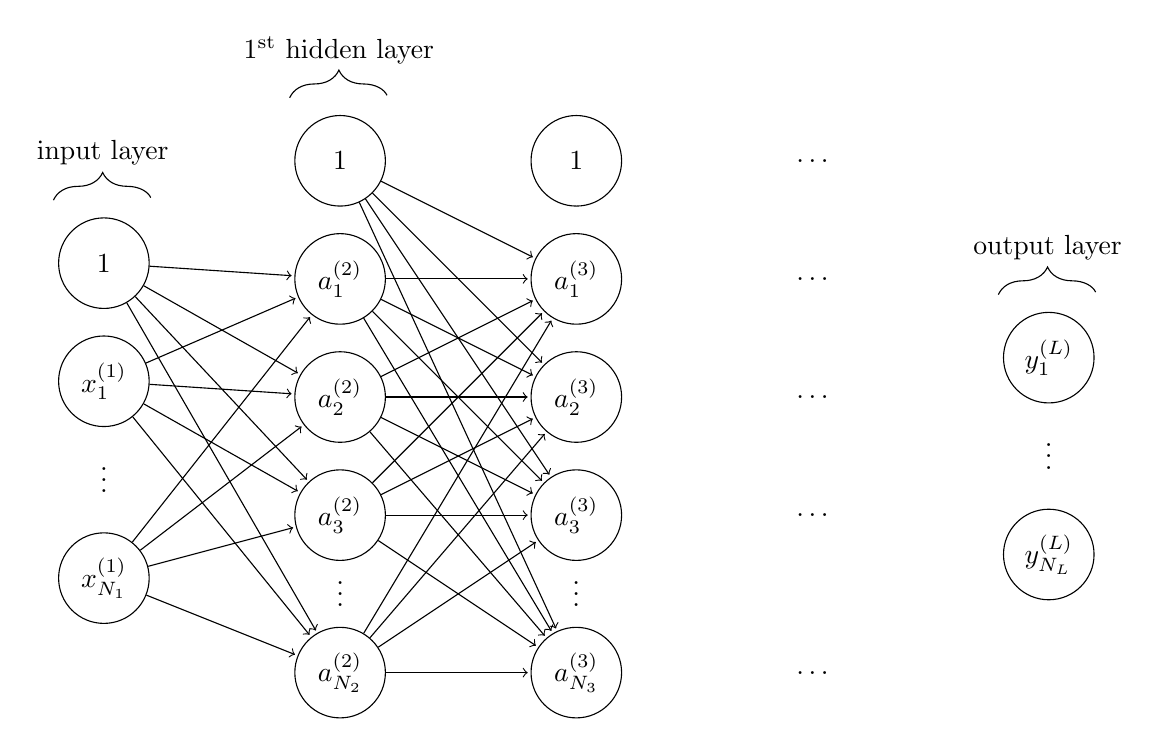
\begin{tikzpicture}[shorten >=1pt]
		\tikzstyle{unit}=[draw,shape=circle,minimum size=1.15cm]
		%\tikzstyle{hidden}=[draw,shape=circle,fill=black!25,minimum size=1.15cm]
		\tikzstyle{hidden}=[draw,shape=circle,minimum size=1.15cm]
		
		\node[unit](1x1) at (0,5.2){$1$};
		\node[unit](x11) at (0,3.7){$x_1^{(1)}$};
		\node at (0,2.55){\vdots};
		\node[unit](x1N) at (0,1.2){$x_{N_1}^{(1)}$};
		
		\node[hidden](1x2) at (3,6.5){$1$};
		\node[hidden](x21) at (3,5){$a_1^{(2)}$};
		\node[hidden](x22) at (3,3.5){$a_2^{(2)}$};
		\node[hidden](x23) at (3,2){$a_3^{(2)}$};
		\node at (3,1.1){\vdots};
		\node[hidden](x2N) at (3,0){$a_{N_2}^{(2)}$};
		
		\node[hidden](1x3) at (6,6.5){$1$};
		\node[hidden](x31) at (6,5){$a_1^{(3)}$};
		\node[hidden](x32) at (6,3.5){$a_2^{(3)}$};
		\node[hidden](x33) at (6,2){$a_3^{(3)}$};
		\node at (6,1.1){\vdots};
		\node[hidden](x3N) at (6,0){$a_{N_3}^{(3)}$};
		
		\node(d5) at (9,0){$\ldots$};
		\node(d4) at (9,2){$\ldots$};
		\node(d3) at (9,3.5){$\ldots$};
		\node(d2) at (9,5){$\ldots$};
		\node(d1) at (9,6.5){$\ldots$};
		
		\node[unit](y1) at (12,4){$y_1^{(L)}$};
		\node at (12,2.85){\vdots};	
		\node[unit](yN) at (12,1.5){$y_{N_L}^{(L)}$};
		
		\draw[->] (1x1) -- (x21);
		\draw[->] (1x1) -- (x22);
		\draw[->] (1x1) -- (x23);
		\draw[->] (1x1) -- (x2N);
		\draw[->] (x11) -- (x21);
		\draw[->] (x11) -- (x22);
		\draw[->] (x11) -- (x23);
		\draw[->] (x11) -- (x2N);
		\draw[->] (x1N) -- (x21);
		\draw[->] (x1N) -- (x22);
		\draw[->] (x1N) -- (x23);
		\draw[->] (x1N) -- (x2N);
		
		\draw[->] (1x2) -- (x31);
		\draw[->] (1x2) -- (x32);
		\draw[->] (1x2) -- (x33);
		\draw[->] (1x2) -- (x3N);
		\draw[->] (x21) -- (x31);
		\draw[->] (x21) -- (x32);
		\draw[->] (x21) -- (x33);
		\draw[->] (x21) -- (x3N);
		\draw[->] (x22) -- (x31);
		\draw[->] (x22) -- (x32);
		\draw[->] (x22) -- (x33);
		\draw[->] (x22) -- (x3N);
		\draw[->] (x23) -- (x31);
		\draw[->] (x23) -- (x32);
		\draw[->] (x23) -- (x33);
		\draw[->] (x23) -- (x3N);
		\draw[->] (x2N) -- (x31);
		\draw[->] (x2N) -- (x32);
		\draw[->] (x2N) -- (x33);
		\draw[->] (x2N) -- (x3N);
		
		\draw [decorate,decoration={brace,amplitude=10pt},xshift=-4pt,yshift=0pt] (-0.5,6) -- (0.75,6) node [black,midway,yshift=+0.6cm]{input layer};
		\draw [decorate,decoration={brace,amplitude=10pt},xshift=-4pt,yshift=0pt] (2.5,7.3) -- (3.75,7.3) node [black,midway,yshift=+0.6cm]{$1^{\text{st}}$ hidden layer};
		\draw [decorate,decoration={brace,amplitude=10pt},xshift=-4pt,yshift=0pt] (11.5,4.8) -- (12.75,4.8) node [black,midway,yshift=+0.6cm]{output layer};
		\end{tikzpicture}
		\caption{Graph of an $L$-layer network with $d = N_1$ input units and $c = N_L$ output units. The $l^\mathrm{th}$ hidden layer contains $N_l$ hidden units and a bias.}
	\end{figure}
	
	
	%\bibliography{/Users/matthewoshaughnessy/Documents/Research/moshaughnessy}
	
\end{document}
